% Packages
\documentclass[11pt,a4paper]{article}
\usepackage[utf8]{inputenc}
\usepackage[T1]{fontenc}
\usepackage{hyperref}
\usepackage{lmodern}
\usepackage[english]{babel}
\usepackage{appendix}
\usepackage{enumitem}
\usepackage{xcolor}

%Fusionneer des pages
\usepackage{pgfpages}
%\pgfpagesuselayout{4 on 1}[a4paper,border shrink=5mm]

% Taille marges
\usepackage[left=2cm,right=2cm,top=2cm,bottom=2cm]{geometry}
% Titles size
\usepackage{titlesec}

% math
\usepackage{amsfonts}
\usepackage{amsmath}
\usepackage{amssymb}
\usepackage{mathabx}
\usepackage{stmaryrd}

\begin{filecontents*}{Annexe 1}
[NEAT]
fitness_criterion     = max
fitness_threshold     = 10000
pop_size              = 500
reset_on_extinction   = False

[DefaultGenome]
# node activation options
activation_default      = tanh
activation_mutate_rate  = 0.2
activation_options      = sigmoid tanh relu

# node aggregation options
aggregation_default     = sum
aggregation_mutate_rate = 0.0
aggregation_options     = sum

# node bias options
bias_init_mean          = 0.0
bias_init_stdev         = 1.0
bias_max_value          = 30.0
bias_min_value          = -30.0
bias_mutate_power       = 0.5
bias_mutate_rate        = 0.7
bias_replace_rate       = 0.1

# genome compatibility options
compatibility_disjoint_coefficient = 1.0
compatibility_weight_coefficient   = 0.5

# connection add/remove rates
conn_add_prob           = 0.5
conn_delete_prob        = 0.3

# connection enable options
enabled_default         = True
enabled_mutate_rate     = 0.01

feed_forward            = True
initial_connection      = full
#full_nodirect

# node add/remove rates
node_add_prob           = 0.2
node_delete_prob        = 0.2

# network parameters
num_hidden              = 0
num_inputs              = 8
num_outputs             = 9

# node response options
response_init_mean      = 1.0
response_init_stdev     = 0.0
response_max_value      = 30.0
response_min_value      = -30.0
response_mutate_power   = 0.0
response_mutate_rate    = 0.0
response_replace_rate   = 0.0

# connection weight options
weight_init_mean        = 0.0
weight_init_stdev       = 1.0
weight_max_value        = 30
weight_min_value        = -30
weight_mutate_power     = 0.5
weight_mutate_rate      = 0.8
weight_replace_rate     = 0.1

[DefaultSpeciesSet]
compatibility_threshold = 3.0

[DefaultStagnation]
species_fitness_func = max
max_stagnation       = 15
species_elitism      = 3

[DefaultReproduction]
elitism            = 3
survival_threshold = 0.2
\end{filecontents*}
\begin{filecontents*}{Annexe 2}
    batch_size = 40
    epochs = 5000
    max_episode_duration = 1000 * 1/env.env.time
    epsilon_max = 1
    epsilon_min = 0.01
    epsilon_decay = 30.
    lr = 1e-4
    discount_factor = 0.9
    self.model = DQN(400,8,self.n_action)
\end{filecontents*}
\usepackage[most]{tcolorbox}
\newtcolorbox[auto counter]{definition}[1]{colframe=red!75!black, coltitle=white, enhanced, frame empty, colback=white,fonttitle=\bfseries , title=Def \thetcbcounter$\;$: #1, borderline west={2pt}{0pt}{red!85!black},
attach boxed title to top left={xshift=-5mm}, boxed title style={colback=red!75!black}}

\newtcolorbox[auto counter]{prop}{colframe=black!80!white, coltitle=black, enhanced, frame empty, colback=white,fonttitle=\bfseries , title=\underline{Property \thetcbcounter$\;$:}, borderline west={2pt}{0pt}{black},
attach boxed title to top left={xshift=-4mm}, boxed title style={frame empty,colback=white}}

\newtcolorbox[auto counter]{thm}[1]{colframe=blue!70!black,colback=white,fonttitle=\bfseries , title=Theorem \thetcbcounter$\;$: #1}

\newtcolorbox[auto counter]{exercice}{colframe=white,colback=white,fonttitle=\bfseries , title=Exercice \thetcbcounter$\;$:}

\newtcolorbox{preuve}{boxrule=0pt, enhanced, colback=white, colframe=white, coltitle=black, fonttitle=\bfseries , title=\underline{Proof $\;$:},
top=0mm, frame empty, borderline west={1pt}{0pt}{black}, sharp corners,
after upper={\par\hfill\textit{$\blacksquare $}}}

\newtcolorbox{mybox}{colframe=white!75!black,colback=white!95!black,fonttitle=\bfseries}

% pseudo code
\usepackage[ruled,lined,noend]{algorithm2e}
\usepackage{babel}

% insertion image
\usepackage{graphicx}
\graphicspath{ {./images/} }

% derivation tree
\usepackage{ebproof}

% automate
\usepackage{caption}
\usepackage{tikz}
\usetikzlibrary{automata, positioning, arrows, decorations.pathreplacing, decorations.markings, positioning, shapes, quotes}


\newcounter{fig}
\newcommand{\fig}[3]{
	\begin{center}
	\begin{figure}[ht]
		\refstepcounter{fig}
		\centering
		\begin{tikzpicture}[scale=#3]
		#1
		\end{tikzpicture}
		\caption{\underline{#2}}
	\end{figure}
	\end{center}
}

\newcommand{\tab}{\phantom{xxx}}

\newcommand{\ignore}[1]{}

\newcommand{\uao}[3]{\underset{#1}{\overset{#2}{#3}}}

\renewcommand{\lim}[2]{\underset{#1 \rightarrow #2}{lim}}

\newcommand{\mlist}[1]{\begin{itemize}[noitemsep,topsep=0pt]#1\end{itemize}}



\title{\huge{\vspace{-1.0cm}Performance Evaluation project:\\\underline{Optimizing cars' trajectory with AI}}}
\date{}
\author{\vspace{-1cm}Ottavy Macéo, Longatte Mathieu, Mocq Louison}

\begin{document}
\maketitle
%\tableofcontents
\titleformat*{\section}{\huge\bfseries}
\titleformat*{\subsection}{\Large\bfseries}


	\section*{Abstract}

The project is divided into five parts:
\mlist{
\item Creating a racing car environment to simulate a simple 2D racing car model.
\item Implementing Deep Q-Learning and Genetic Algorithms to optimize the behavior of a car on every possible tracks, enabling it to follow the best possible trajectories.
\item Evaluating the performance of Deep Q-Learning and Genetic Algorithms and comparing their results.
\item Assessing the performance of Deep Q-Learning with respect to different hyper-parameters.
\item Evaluating the performance of the best car behavior achieved by both algorithms.
}
You can see the complete project on our public \href{https://github.com/GeckSpy/PE-trajectory-optimization}{Github page}.
% All the code has been developed in Python.

	\section*{Introduction}

We focus on solving the problem of optimizing a car's trajectory using a Deep Q-Learning model. 
The goal is to assess the ability of this model to generalize its experience from a limited number of circuits to new ones. 
To achieve this, we consider the car's trajectory in a plane under a simplified physics model. 
The model's performance will be compared to that of a genetic algorithm. 
Then, we will examine the impact of the chosen hyper-parameters on the model's training performance. 
Finally, we will explore the model's limitations when trained on a large amount of data.

	\section*{Modeling}
		\subsection*{Racing environment}
			\subsubsection*{Tracks}
A track is originally a .png file as shown by the first image of figure \ref{figure:track}.
 Then, the image is converted to a matrix $T$ such that $T[0][0]$ is the bottom left corner. 
 Finally, we crop the image, compute the starting point, and determine the lines of the track (these will be explained in the reward section) to obtain the final result shown by figure \ref{figure:track}. 
 

\begin{center}
	\begin{figure}[ht]
		\centering
		
\includegraphics[width=5cm, height=4cm]{track_06.png}
		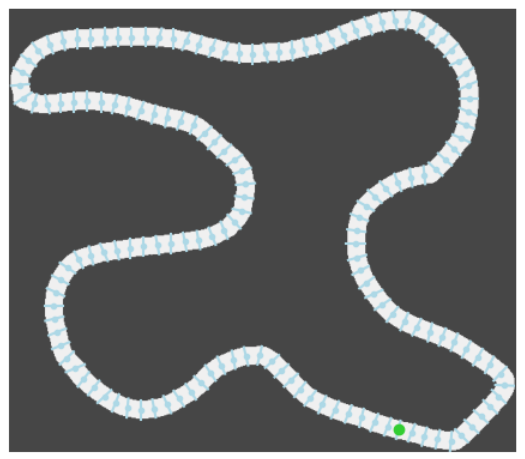
\includegraphics[width=5cm, height=4cm]{track_06_computed.png}
		\caption{\underline{Before and after processing the track :} the white squares represent the road, and the green point represents the starting point }
		\label{figure:track}
	\end{figure}
\end{center}
	
			\subsubsection*{Car's physics}
The car's physics model is quite simple, it follows a 2D cartoon-like set of physical laws :
\begin{itemize}
    \item The car is characterized by two main properties: its speed $s \in [0, \text{MaxSpeed}]$ and its direction $\alpha \in [0, 360]$
    \item The physical laws work as follows: at each time step, the car moves in the direction defined by $\alpha$, covering a distance equal to its speed.
    \item If the current coordinates are $(x, y)$, its speed is $s$, and its direction is $\alpha$, then after one time step, the new coordinates of the car will be:
    \[
    (s \cdot \cos\left(\frac{\pi}{180}\alpha\right) + x,\; s \cdot \sin\left(\frac{\pi}{180}\alpha\right) + y)
    \]
\end{itemize}


Moreover, at each time step, the car will take an action:
\mlist{
\item It can accelerate, this will increase the car's speed by a constant.
\item It can brake, this will decrease the car's speed by a constant. Note that the car cannot have a negative speed, it means that it cannot go backward.
\item It can turn, i.e. add a constant $\in \llbracket-K,K\rrbracket$ to its rotation. $K$ is a constant that is the maximum angle the car can turn per time step.
}
\tab \\
The car needs to interact with the track, therefore we need to decide what is the state of a car, i.e, what the car knows about the environment. 
We could model a state by the matrix of the track and the information of the car but this would lead to a state of large dimension because a track can have size $900\times600$ pixels. Moreover, it will be hard to train from those states because there is a great diversity of possible tracks. 
To reduce the dimension of the problem, we decided to represent a state as a real car racer would see it. Then, the state of a car is an array $V$ of size $8$.
\mlist{
\item $V_0$ is the current speed of the car
\item $\forall i\in\{1,...,7\}$, $V_i$ is the distance of the car to the next wall in the direction $\alpha + A_{i-1}$ where $\alpha$ is the current rotation of the car and $A=[60, 40, 20, 0, -20, -40, -60]$
}
Then, a typical state is represented by the figure \ref{figure:car state}.
\begin{center}
	\begin{figure}[ht]
		\centering
		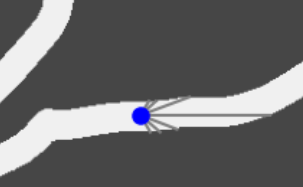
\includegraphics[width=4cm, height=3cm]{car_state.png}
		\caption{\underline{Car state}}
		\label{figure:car state}
	\end{figure}
\end{center}
		
			\subsubsection*{Technical aspects of the environment}
To manipulate our environment, we use the python packages \texttt{gymnasium} which provides code conventions for Markov decision process environments (i.e. environment in which at each time step you have to take an action and receive a reward). 
The environment must have some essential methods: \texttt{reset()} that resets the environment in order to begin a new simulation, \texttt{render()} that renders the current state of our environment, 
and \texttt{step()} that does one step of time, i.e. given an action, the \texttt{step()} function figure out is the car has crashed or not, move the car to its next position and return the new state of the car, a reward and if the car has crashed.\\
Finally, the environment has a variable \texttt{time} which measures how much time is discretized
		
			\subsubsection*{Rewards}
For those type of problem where the AI model has to compute a behavior, the AI model produces something which look like a function $f$ that take a car state and return an action. We need to specifies to our AI model when it produce a good action and a bad action, for instance, if a car crash, we need to punish the AI model.\\
We do that thanks to a reward function implemented in the function \texttt{step()} of our environment. The reward is an integer, the bigger it is the best the action was. This function is clearly the most important one of all the project because it is thanks to it that our AI model will perform well or not. We tried lot of reward functions, some that we invent, other that we see on other projects and we finish by using the following one:\\
\\
To punished the car when it do something bad we do:
\mlist{
\item If the car crashes, we stop the simulation and return a reward of $-500$.
\item If the car is not moving, i.e. has a speed of $0$, the reward is $-10$.
}
For the positive reward, we have automatically computed some track line thanks to an algorithms we ceated (represented in right image of figure \ref{figure:track}). If the car crosses next line, it has a reward of $(+10\times$ the number of lines it has cross in the good order with this action). If the car cross a line in the wrong order, it means that it has gone backward, therefore, we punished the car with a reward of $-200$ and we stop the computation.\\
On top of that, at each time step, we add to the current reward the speed of the car divided by a constant to encourage the car to go fast. Finally, we subtrack the reward by $1$ to encourage the car to cross has many lines has possible with the least amout of time steps.

			\subsubsection*{An example of a car on a track}
After explaining all of this, here is an example in figure \ref{figure:env example}. We have plot the trajectory of the car, the green color is when the car has accelerate, red color when it has brake and yellow otherwise.
\begin{center}
	\begin{figure}[ht]
		\centering
		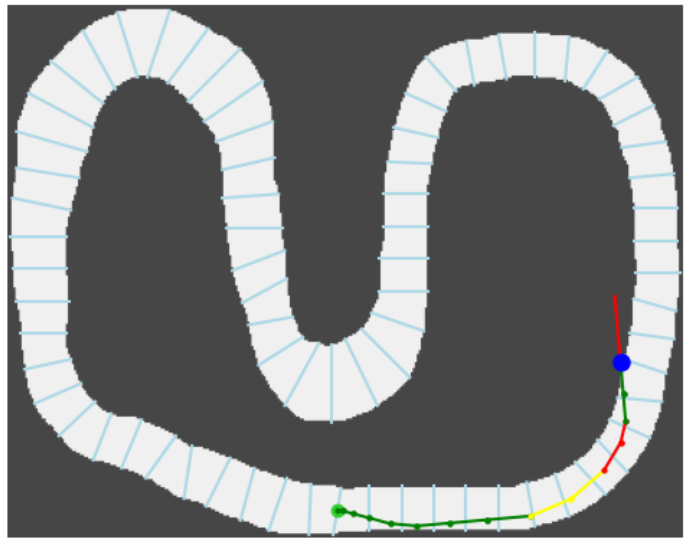
\includegraphics[width=6cm, height=5cm]{env_example.png}\\
		List of rounded reward: $R=$\texttt{[10, 1, 2, 12, 13, 13, 13, 14, 24, 14, 13, 12, 13, -497]}
		\caption{\underline{Car state}}
		\label{figure:env example}
	\end{figure}
\end{center}
The total reward of a car behavior is the sum of all reward of a simulation with a car behavior. For example, the reward of the car behavior or the figure \ref{figure:env example} is $\underset{r \in R}{\sum} r= -343$.


		\subsection*{Deep Q-learning}
Deep Q-Learning is a reinforcement learning algorithm that combines Q-Learning with Deep Learning to solve complex decision-making problems. It allows an agent to learn how to act optimally in environments with large state spaces by approximating a function, known as the \textit{Q-function}, which evaluates the quality of an action taken in a given state.
    
            \subsubsection*{Q-function}
The Q-function, $Q(s, a)$, represents the expected cumulative reward an agent will receive after taking action $a$ in state $s$, and then following the optimal policy. The cumulative reward is computed as:
\[Q(s, a) = r + \gamma \max_{a'} Q(s', a'),\]
Where:
\mlist{
\item $r$ is the immediate reward received after taking action $a$ in state $s$.
\item $s'$ is the next state reached.
\item $a'$ is the next action.
\item $\gamma \in [0, 1]$ is the discount factor, which balances immediate and future rewards.
}
    
            \subsubsection*{Key Techniques}
\mlist{
    \item \textbf{Replay Buffer}: A memory that stores past experiences $(s, a, r, s')$. Randomly sampling experiences from the buffer during training reduces correlations between consecutive samples, improving learning stability.
    \item \textbf{Exploration-Exploitation Balance}: The agent uses an $\varepsilon$-greedy policy to choose actions, where it explores randomly with probability $\varepsilon$ and exploits the best-known action otherwise.
}
    
            \subsubsection*{High-Level Workflow}
\mlist{
\item Observe the current state $s$.
\item Choose an action $a$ using an $\varepsilon$-greedy policy.
\item Execute the action, observe the reward $r$ and next state $s'$.
\item Store the experience $(s, a, r, s')$ in the replay buffer.
\item Sample a mini-batch of experiences from the buffer to train the Q-network.
}
    


	
		\subsection*{Genetic algorithms}
			\subsubsection*{What are genetic algorithms?}
Genetic algorithms (GA) are probabilistic algorithms based on natural selection. Therefore, GA takes some \textbf{populations} which are sets of solutions (here a solution is a car's behavior), select the best solutions thanks to the reward function. Then, it changes the population by adding new random solutions, adding some \textbf{mutations} which are some small variations of a behavior, adding some \textbf{cross-over} which are the equivalent of natural reproduction. We can either repeat this process a fixed number of generations or for a fixed amount of time.
		
			\subsubsection*{Markov Chain modernization}
We will now introduce a Markov chain modelization for genetic algorithm. We define a Markov chain $(Y_n)_{n\in\mathbb{N}}$ as following:
\mlist{
\item A state of $(Y_n)_{n\in\mathbb{N}}$ is a population.
\item Let $y_0$ be a special state such that if $Y_n = y_0$ then it means that the population of state $Y_n$ contain an optimal solution.
}
\tab \\
Now, the sequence of population of genetic algorithm can be describe with this Markov chains. $Y_n$ represent the population at generation $n$. Notice that the state $y_0$ is an absorbing state. In fact if $Y_n = y_0$ then it mean that the population $P_n$ contain an optimal solution. Since we always keep the best solution of the previous population, it means that $\forall n'>n$, we have that $P_{n'}$ contain an optimal solution. Therefore, $\forall n'>n$, $Y_{n'} = y_0$. Moreover, $y_0$ is the only absorbing state of $(Y_n)_{n\in\mathbb{N}}$.\\
\\
If we suppose that our mutation and cross-over are made such that a solution $x$ can reach $y$ by a series of a finite number of those operations, then, all solutions $x$ can reach an optimal value. Then every state $y_n$ can reach the state $y_0$. The set of all possible state is finite. Then $\mathbb{P}(Y_n = y_0) \underset{n \rightarrow +\infty}{\rightarrow} 1$\\
Then $\mathbb{P}($ The population $P_n$ contain an optimal solution$) \underset{n \rightarrow +\infty}{\rightarrow} 1$.\\
Thus, the genetic algorithm converge toward a global optimal solution. However, we do not know how many time it will take in average.
		
			\subsubsection*{NEAT}
Basic genetic algorithms are not efficient enough to compute an optimized behavior. Therefore, we will use the famous python packages called \texttt{NEAT}. It is an optimized generalized genetic algorithms with represent solution as dynamic neural network. By dynamic we mean that the algorithm can add or delete some of the nodes of the neural network. The principle of GA stay the same but we have a lot more hyper-parameters.
	
	
	\section*{Simulation}
Once we completed the modeling of the environment, the deep Q-learning algorithm and the genetic algorithm, we have to compute some simulation to process evaluation performance. We will compare our two algorithms using various metrics. For this purpose, we choose the following metric: the average reward after training depending of some parameter, we call it the score of a training. We measure this value across different training durations and varying the numbers of tracks used to training the models. To ensure robustness and evaluate potential over-fitting, we test the models on tracks that were not included in the training set.\\
This approach is applied in the context of an AI project where we train AI agents to complete a racing circuit. The goal is for the cars to complete laps as quickly as possible, and the average reward reflects their performance under these conditions.
\mlist{
\item First, we will compare genetic algorithm to Q-learning depending of the training time and the number of tracks used to train the car. We will train our algorithms during $10$ to $60$ minutes and with $10$ to $67$ tracks (which represent $80\%$ of the total number of tracks created).
\item Then, we will compare the result of deep Q-learning depending of some hyper-parameters. The goal here is to be able to find the hyper-parameters that fit the most the situation, and for us this evaluation is only possible by running the algorithms with different parameters.
\item Finally, we will evaluate the performance or the best car we found using deep Q-learning.
}

    \section*{Experimental}
All the computations presented in this section were performed on the \href{https://www.grid5000.fr}{Grid5000} infrastructure, which allowed us to ensure the reproducibility of the results and guarantee a consistent comparison of the executions, as they were carried out on machines with equivalent performance and assure stability of our executions.

		\subsection*{Comparison between Deep Q-Learning and Genetic Algorithm}
Firstly, our goal was to be able to compare the different models we tried to use to train the car, in order to do that, we choose to give a certain time and a certain amount of tracks for the different models. The models were allowed to be training for this amount of time on \href{https://www.grid5000.fr}{Grid5000}.\\
We choose to evaluate the models on these metrics because we believed that they were the most important in the training of such AI. Indeed, these metrics allow the users to have an idea on how powerful can the models be.\\
As said before, we choose to evaluate the average reward on tracks on which the car has not trained, we believed it is the most relevant way to evaluate the training because it allows us to evaluate if there is over-fitting or not and this represent how much the car is doing well on the track.\\
\\
Since the training can be long to have satisfying result, we choose to concentrate ourselves on the following durations : $\{10;40;60\}$ (minutes) and the following number of tracks for the training $\{10;40;67\}$ (tracks). We evaluate these trainings on $20$ tracks that are not in the training set. The two models are run with specific hyper-parameters for this section that are described in the final section \pageref{Hyperparameters}. The result are in figure \ref{figure:compare GA VS DQ}.
        \begin{figure}[ht]
            \centering
            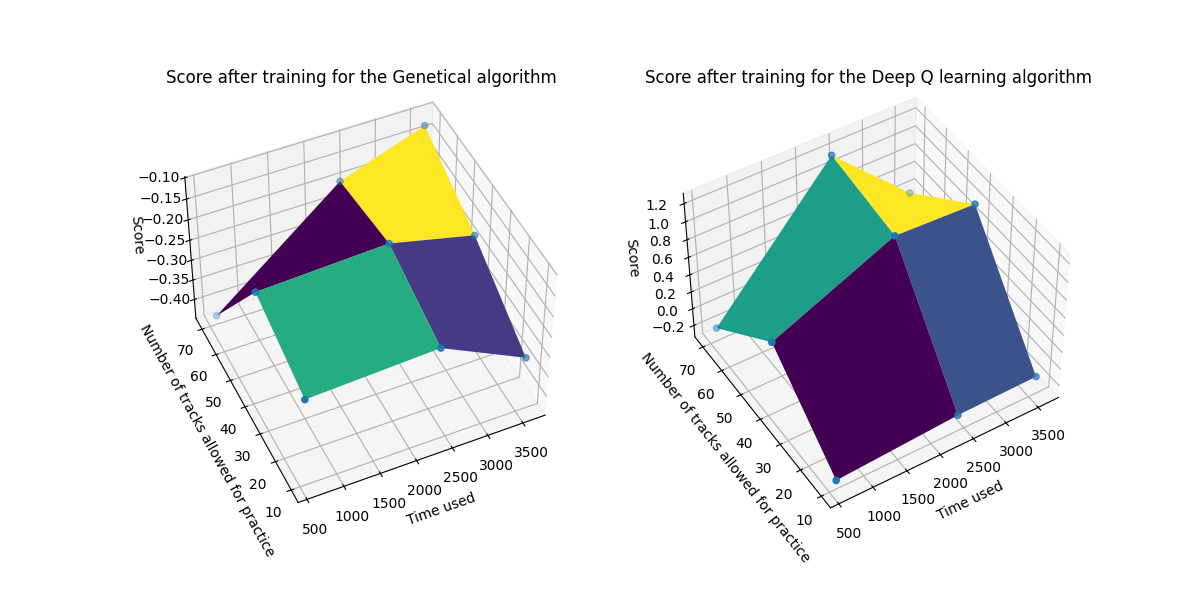
\includegraphics[scale = 0.65]{graphe_comparaison.png}
            \caption{Comparison between the Genetic algorithm and the Deep Q learning algorithm.}
            \label{figure:compare GA VS DQ}
        \end{figure}

We can notice that the Deep-Q algorithm outperform the Genetic algorithm for every test. We can also notice that sometimes the use of more time or more tracks can lower the performance or our deep Q-learning algorithm. This is surely due to over-fitting.\\
\\
To compare the models, we can also look at the global volatility of the solutions, this represent the standard deviation of score of the training. In order for the algorithm to perform efficiently, we want it to have low standard deviation. The result are shown in figure \ref{figure:standard deviation}.
        \begin{figure}[ht]
            \centering
            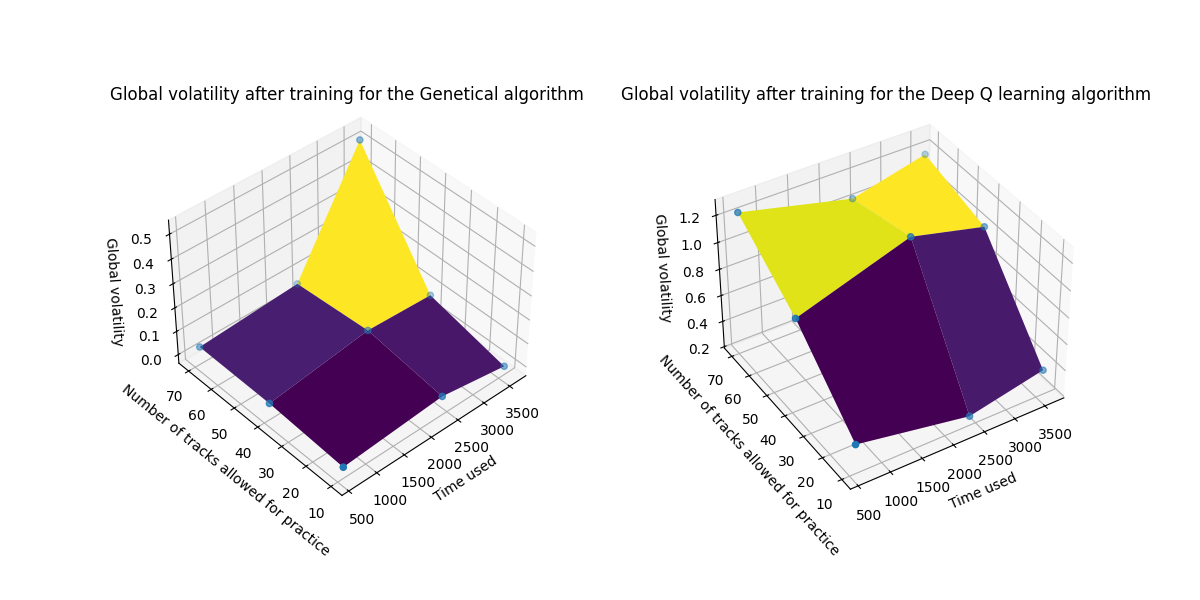
\includegraphics[scale = 0.55]{comparaison3.png}
            \caption{Standard deviation after training}
            \label{figure:standard deviation}
        \end{figure}
 
\newpage
Finally, we can look at the evolution of the reward for the Deep Q learning for $60$ minutes of training on $67$ tracks to have an idea the possible over-fitting happening for this training (figure \ref{figure:evolution of the reward}). We can see that the reward does start decreasing after $650$ generations, this can be a sign of over-fitting.
        \begin{figure}[ht]
            \centering
            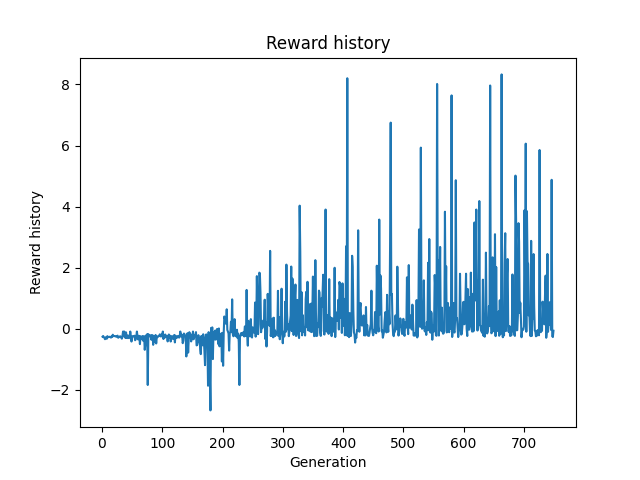
\includegraphics[width=0.5\linewidth]{graphe_reward.png}
            \caption{Evolution of the reward}
            \label{figure:evolution of the reward}
        \end{figure}
        
        
		\subsection*{Influence of Hyper-parameters on Deep Q-Learning}
Focusing on the Deep Q algorithm, we can ask ourselves what are the best hyper-parameters. We focused on $3$ hyper-parameters that we perceived as more important in our model:
\mlist{
\item Batch size : this is the number of samples that are kept in memory between each step of the training. 
\item Lr (learning rate) : this is the velocity at which the neural network update the weights. 
\item Epsilon Decay : this is the probability that the model will try to explore new ways. 
}
We get the following results (figure \ref{figure:Evolution of score depending of hyper-parameter}). These graphs allows us to have an idea on how efficient each hyper-parameter tested is. For example for batch size, we want to have a batch size of $60$ in order to be efficient.
        \begin{figure}[ht]
            \centering
            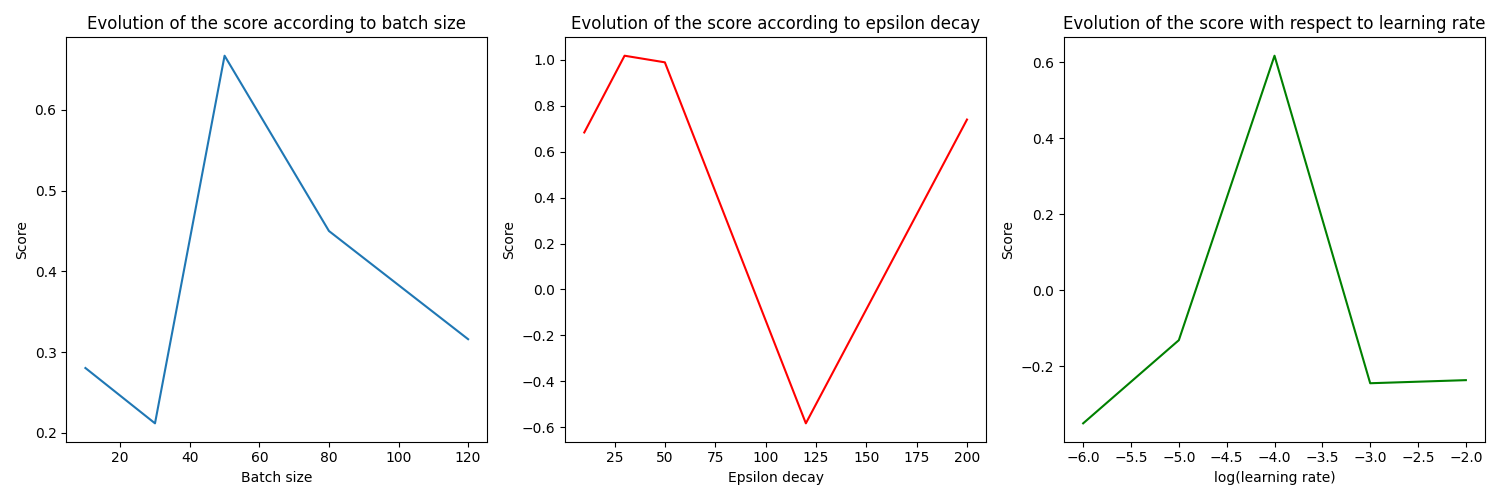
\includegraphics[scale = 0.46]{comparaison2.png}
            \caption{Evolution of the score after fluctuating hyper-parameters}
            \label{figure:Evolution of score depending of hyper-parameter}
        \end{figure}
        
        
        
		\subsection*{Best Car: performances of a model trained for few hours }
        We can now look at the performance of the best car, it is chosen on how efficient it is on the tracks. Firstly, as seen in part one, training for too long on a reduced amount of tracks can lead to over-fitting, we have been able to see this also by training a model for $6$ hours in the same conditions as the other. This model performs way less than the others. We choose the Hyper-parameters chosen thanks to part 2 and the time and number of tracks that maximize the score. You can see on figure \ref{figure:Evolution of best car} the evolution of the car on a map that the car has never seen before. 
        \begin{figure}[h]
            \centering
            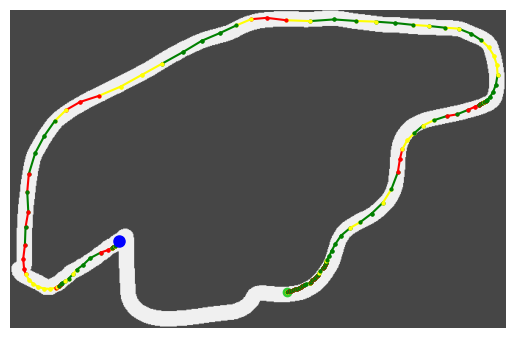
\includegraphics[width=0.5\linewidth]{image.png}
            \caption{Evolution of the best car}
            \label{figure:Evolution of best car}
        \end{figure}
    
    
    \section*{Conclusion}
The goal of the project was to train an AI model to choose the best trajectory for a car on random tracks. To carry out this project, we created an environment to model the evolution of a car on different tracks, then we tried to use different types of training to learn how to use the training algorithm. In particular, we chose the genetic algorithm and the Deep Q-learning algorithm. Finding a relevant reward function for the algorithm was a main part of the work, then evaluating the algorithm allowed us to choose the best hyper-parameters for our models as well as the best training time and number of tracks. Our goal was to be able to compare the performance of the algorithm used and we believe that using the score and global volatility were relevant measures. Initially, we wanted to compare the performance of the algorithms with real performances, 
    this would allow us to keep a foot in reality and to be able to have an idea of the relevance of our work. However, this seems to be much more complicated but it could be an interesting extension of our work.

\newpage
\section*{Appendix}
\subsection*{Reproducibility}
This section store the data necessary to reproduce the experiments: \subsubsection*{Comparison between the Genetic algorithm and the Deep Q learning algorithm.}
Hyper-parameters for the genetic algorithm for part 1.
\begin{mybox}
    \tiny{
\lstinputlisting{Annexe 1}}
\end{mybox}
\label{Hyperparameters}
Hyper-parameters for the Deep Q learning algorithm for part 1.
\begin{mybox}
    \tiny{
\lstinputlisting{Annexe 2}}
\end{mybox}

\end{document}